\documentclass[8pt]{extarticle}

\usepackage{listings}
\usepackage[thinc]{esdiff}
\usepackage{amsmath}
\usepackage{commath}
\usepackage{biblatex}
\usepackage{fouriernc,bm}
\usepackage{multicol}
\usepackage{changepage}
\usepackage[font=small]{caption}
\usepackage{geometry}
\usepackage{xcolor}

\usepackage{graphicx}
\graphicspath{ {./image} }

\geometry{left=18mm, right=18mm, top=20mm}
  \setlength\columnsep{30pt}
 
\definecolor{codegreen}{rgb}{0,0.6,0}
\definecolor{codegray}{rgb}{0.5,0.5,0.5}
\definecolor{codepurple}{rgb}{0.58,0,0.82}
\definecolor{backcolour}{RGB}{251,251,251}

\lstdefinestyle{mystyle}{
    backgroundcolor=\color{backcolour},   
    commentstyle=\color{blue},
    keywordstyle=\color{magenta},
    numberstyle=\tiny\color{codegray},
    stringstyle=\color{codepurple},
    basicstyle=\fontencoding{T1}\footnotesize\fontfamily{lmtt}\fontseries{s}\selectfont,
    breakatwhitespace=false,         
    breaklines=true,                 
    captionpos=b,                    
    keepspaces=true,                 
    numbers=left,                    
    numbersep=5pt,                  
    showspaces=false,                
    showstringspaces=false,
    showtabs=false,                  
    tabsize=4,
    frame=single
    morekeywords={__global__, __device__},  % CUDA specific keywords
}

\lstset{style=mystyle}

\begin{document}

\begin{small}

\newpage

\begin{multicols}{2}



\section{workflow}

\begin{lstlisting}[language=bash]
#------------#
# TMUX-SHELL #
#------------#

$ C-l							# clear screen		
$ C-w							# delete word
$ C-_							# undo
$ C-c							# kill		
$ C-d							# exit
$ C-Z							# suspend process
$ fg							# restore process
$ C-a							# jump to the strt of the line
$ C-e							# jump to the end of the line
$ open <directory path>			# open in finder
#-----------------------------------------------------------#
$ C-space ""					# split pane
$ C-space %						# split pane
$ C-space arrow					# jump panw
$ C-space {						# move pane
% C-space }						# move pane
$ C-space x						# kill pane
$ C-space q						# show pane number
$ C-space q 1					# goto pane 1

$ :resize-pane -D 				# resizes down 
$ :resize-pane -U 				# resizes upward 
$ :resize-pane -L 				# resizes left 
$ :resize-pane -R 				# resizes right 
$ :resize-pane -D 10 			# resizes down by 10 cells
$ :resize-pane -U 10 			# resizes upward by 10 cells
$ :resize-pane -L 10 			# resizes left by 10 cells
$ :resize-pane -R 10 			# resizes right by 10 cells
#-----------------------------------------------------------#
$ C-space s						# list session
$ C-space :new					# new session
$ tmux kill-session -t <name>	# kill session
$ tmux attach -t <name>			# re-attach session
#-----------------------------------------------------------#
$ ssh hostname 					# hostname-c_user SSH port22
$ ssh -i foo.pem hostname      	# hostname-identity file
$ ssh user@hostname            	# hostname-user-SSH port22
$ ssh user@hostname -p 8765   	# hostname-user-custom port
$ ssh ssh://user@hostname:8765 	# hostname-user-custom port
$ scp .txt ubuntu@hostname:/home# copy foo.txt into remote dir
#-----------------------------------------------------------#
$ cat foo.c						# create file with content	
$ touch foo.c					# create file without content
#-----------------------------------------------------------#
$ mkdir test					# create dir
$ rmdir test					# remove dirgit 

$ cd ../snippets/				# navigate subdir of parnt dir
$ cd ./mmio.h					# navigate curr dir

$ cp ./file.xyz ../target/		# copy into subdir of parent
$ mv Makefile Makefile_ex		# rename old->new
$ mv * ../						# move all upper folder

$ &&							# chain command in bash
$ pwd							# get location of current dir
$ find /root/sid/ -name "*matrix*"	# search for file
$ rm -rf spmv_openmp			# force remove
$ cp -R t1/. t2/				# copy content
\end{lstlisting}

\begin{lstlisting}[language=bash]
#------#
# MAKE #
#------#

# compiling with linking in non-default name '-o'
# read.o is dependency
# if timestap changed on read.o it will be re-linked
read: read.o mmio.o
	cc -fopenmp -O4 -Wall -g read.o mmio.o -o read

# compiling without linking '-c'; 
# multiple pre-requisites used if anyhting changed
# -Wall gives all the warning; -g turns on the debugger
read.o: example_read.c ../lib/mmio.c
	cc -fopenmp -O4 -c -Wall -g example_read.c -o read.o
	cc -fopenmp -O4 -c -Wall -g ../lib/mmio.c -o mmio.o

clean:
	rm -f read read.o mmio.o

\end{lstlisting}


\begin{lstlisting}[language=bash]
# 1_login remotely
$ ssh -X sid@crescent.central.cranfield.ac.uk
$ password
$ module load fosscuda/2019b
$ export CC=$(which gcc)

# 2_create source file
$ vim ex1.c
$ vim Makefile

# 3_compile manually / with Make / recompile with Make
# o gives it a custom name instead of default
$ gcc -fopenmp -O4 -o ex1 ex1.c
$ make ex1
cc -Wall -g		ex1.c	-o ex1
$ make clean
rm -f ex1
$ make ex1
cc -Wall -g		ex1.c	-o ex1

# 4_run executable
$ ./ex1
# or add input data and run
$ ./read ../test/cage4.mtx

# 5_create, submit job file
$ vim ex1.sub
$ qsub ex1.sub

# 6_status
$ qstat
$ ls
$ more openMP.02300565

# 7_copy remotely into local
$ scp sid@crescent.central.cranfield.ac.uk:
  openMP.o230565 /Documents/lib/ex2_3.test
\end{lstlisting}


\begin{lstlisting}[language=bash]
#-----#
# GIT #
#-----#

# create a repo on github
# then create a local project folder
$ mkdir SpMV_OpenMP

# initialise git on current folder and push it
$ git init
$ git add README.md
$ git commmit -m "first commit"
$ git branch -M main
$ git remote add origin git@github.com:marcellgyorei/
						spmv_openmp.git
$ git push -u origin main

# or clone repo
$ git clone git@github.com:marcellgyorei/SpMV_OpenMP.git

# check changes have been made before committing
$ git status
# what changes have been made
$ git diff
# see changes on particular file
# which lines have been added/deleted
git diff R/modified.R

# use one global .gitignore whenever check git status
$ nvim ~/.gitignore_global
# add lines into it
*~
.*~
.DS_Store
.Rhistory
.RData
$ git config --global core.excludesfile ~/.gitignore_global

# check log of commits
$ git log
# compressed log
$ git log --pretty=oneline
# commits of certain author
$ git log --author=marcellgyorei
# only files have changed
git log --name-status
# tree log
$ git log --graph --oneline --decorate --all

# drop local changes-commits, fetch latest history from server
$ git fetch origin
$ git reset --hard origin/main

# delete local git repo
$ rm -fr .git
# verify status
$ git status

# delete local folder and re-clone it
$ rm -rf ~/spmv_openmp
$ git clone git@github.com:myname/myproject.git ~/spmv_openmp

# adda a folder content
$ git add foldername/\*

$ git add --all
$ git commit -am "<commit message>"
$ git push

$ git pull --rebase

# is there are unstaged changes list files that prevent pull
$ git status
$ git restore .DS_Store
# delete all local changes
git reset --hard


\end{lstlisting}

\begin{lstlisting}[language=C]
/*----------*/
/* VIM_MODE */
/*----------*/

save as ex1    					:w! ex1
quit/save & quit				:!q		:wq
insert/command mode				i		ESC

/*------------*/
/* VIM_FORMAT */
/*------------*/

indent line forward/backward 	i C-t	i C-d		

/*-----------------------*/
/* VIM_SELECT-COPY-PASTE */
/*-----------------------*/

line selection					V
select word forward/backward 	vw		vb
/*---------------------------------------------------------*/
copy lines by number			:<number>yy
copy current line				yy
copy selection					y
/*---------------------------------------------------------*/
paste buffer before/after crsr	p		P
undo							u

/*-------------*/
/* VIM_REPLACE */
/*-------------*/

replace text					:%s/<match>/<replace>
replace with '					r'
switch case under the char		~

/*------------*/
/* VIM_SEARCH */
/*------------*/

show lines match				[I
/*---------------------------------------------------------*/
search forward/backward			/<match> ?<match>
search word nrst frwrd/bckwrd	*		#
repeat search forward/backward	n		N

/*----------*/
/* VIM_JUMP */
/*----------*/

next/prev page					C-f		C-b
half page up/down				C-u		C-d
/*---------------------------------------------------------*/
top/middle/bottom line			H		M		L
set line numbering				:set number
goto line						:<line number>
/*---------------------------------------------------------*/
to first/last line of a text 	gg		G
/*---------------------------------------------------------*/
end of the line					$	
first char of the line [blank]	0
first char of the line			^
/*---------------------------------------------------------*/
next word						w		W
end of the word 				e		E
prev word						b		B
prev space						F[]
/*---------------------------------------------------------*/
next 'e' char in line			fe
repeat [opposite]				;		,
/*---------------------------------------------------------*/
bracket to bracket				%
left/right/down/up				h		l		j		k

/*------------*/
/* VIM_DELETE */
/*------------*/

until first/last line in text	dgg		dG
bracket content					dt%
/*---------------------------------------------------------*/
current line					dd				cc
current & prev/next line 		dk		dj
until end of the line			d$
/*---------------------------------------------------------*/
start of the word forward		dw		dW		cw
end of the word forward	 		de		dE
start of the word backward		db		dB
/*---------------------------------------------------------*/
until " char					dt"
current	char					x

\end{lstlisting}

\vfill\null
\columnbreak

\section{c++}

\begin{lstlisting}[language=C]
/*------------------*/
/* LEARNING SOURCES */
/*------------------*/

/* REAL-TIME */

1st	C++_2.16__E_Christopher Kormanyos - Real-Time C++ 2021
	[Appendix A - Tutorial page 439 and from chapter 3]

	// vs code
	// compiler explorer
	// aUnx_0.0.1__Setup
	
/* CLEARITY */
	
2nd	C++_2.18__E_Rainer - C++ Core Guidelines Explained 2022
	/**/
ref	C++_1.34__S_ISO_IEC 14882_2020 Sixth edition 2020
ref	C++_2.17__S_Bjarne - CppCoreGuidelines
	
/* CORE BASICS 2020 & STL */

2nd	C++_1.36__E_Pitt - Guide to Scientific Computing 2018
ref	C++_1.31__E_Paul Deitel - C++ for Programmers 2022
ref C++_1.28__E_Hacking C++ - C++ Cheat Sheets & Infogrph STL

/* LOW BUILT-TIME */
/* DATA STRUCTURES, ALGORITHMS */

	C++_2.7__S_Joe Gibson - C++ Data Str & Algo Cheat Sheet

/* TEST */

	C++_2.15__E_Leetcode - C++

/* REQS, DESIGN, SPECS */

	// UML paperback
	// omnigraffle/window/stencil/search uml
	// sketch

/* WHITE-BOARDING */
/* DESIGN TOOL */
/* TRADING TOOL */
\end{lstlisting}


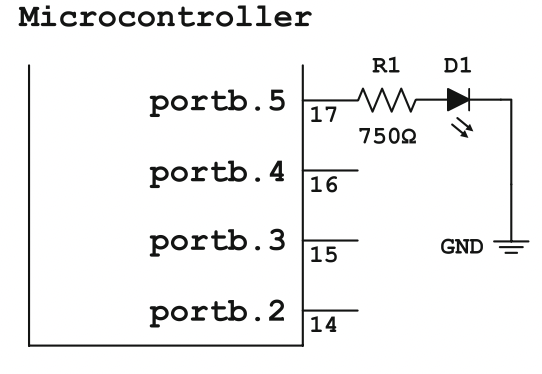
\includegraphics[scale=0.3]{mcontroller}

\begin{lstlisting}[language=C]
/* KORMANYOS - REAL-TIME C++ 2021 */
/* LED PROGRAM [PAGE 4] */

#include <cstdint>
#include "mcal_reg.h"

class led
{
public:
	typedef std::uint8_t port_type;
	typedef std::uint8_t bval_type;
	
	led(const port_type p,
		const bval_type b) : port(p),
							 bval (b)

\end{lstlisting}

\begin{lstlisting}[language=C]
// led.h
class led
{
public:
	led(const port_type p,
		const bval_type b);
	
	void toggle() const;
};	
\end{lstlisting}
\begin{lstlisting}[language=C]
// led.cpp
\end{lstlisting}

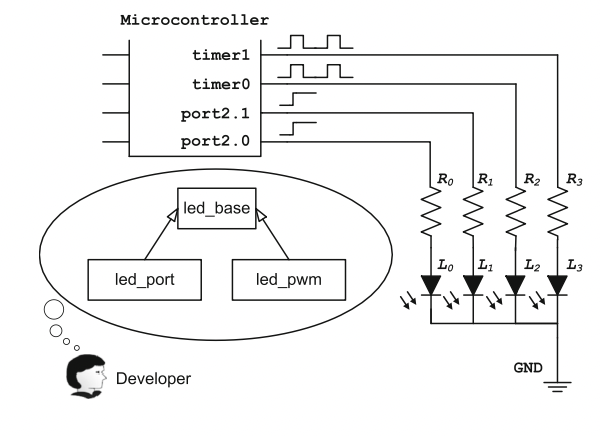
\includegraphics[scale=0.5]{oo_mcontroller}

\begin{lstlisting}[language=C]
/* INHERITANCE [PAGE 76]*/
\end{lstlisting}





\section{c}


%\subsection{//}


\begin{lstlisting}[language=C]
/*-------------------------------*/
/* USER DEFINED FUNCTION EXAMPLE */
/*-------------------------------*/

//  pre-processor directive necessary when using math library
#include <math.h>

//  function prototype
double gen_sqrt(double);

//  main function
int main()
{
	//  variables
    double val,sqroot;
    
    //  ask the user to enter a real number   
	printf("Enter a floating point value > 0");
	
    //  get the value from the user
	scanf("%lf",&val);
	
    //  call the function to compute the generalised sq root
    sqroot=gen_sqrt(val);
    
    //  print out the result
    printf("The generalised square root of %lf is %lf\n",val,
    	   sqroot);
    
    return 0;
}

//  user-defined function gen_sqrt
double gen_sqrt(double x)
{
	double result;
	if(x <0.0)
	{
        result=-sqrt(-x);
	else
	{
		result=sqrt(x);
	}
	return (result);
}
\end{lstlisting}

\begin{lstlisting}[language=C]
/*-----------*/
/* VARIABLES */
/*-----------*/

auto		break		char		double
else		extern		int			return
struct		case		enum		long
register	switch		typedef		union
const		continue	float		for
short		unsigned	default		goto
signed		sizeof		void		do
static		volatile	if			while
\end{lstlisting}

\begin{lstlisting}[language=C]
/*------------*/
/* DATA TYPES */
/*------------*/

Type		PC	Dec MIPS	Dec Alpha		Dec Alpha 
				(OSF/1)		(ULTRIX)		(OPEN VMS)

char		1	1			1			1
short int	2	2			2			2
int			2	4			4			4
long int	4	4			8			4
float		4	4			8			4
double		8	8			8			8
\end{lstlisting}

\begin{lstlisting}[language=C]
/*-----------*/
/* INCREMENT */
/*-----------*/

//  output i: 1
int main()
{
	int i=0;
	printf("i: %d\n",++i);
	return 0;
}

//  output i: 0
int main()
{
	int i=0;
	printf("i: %d\n",i++);
	return 0;
}
\end{lstlisting}

\begin{lstlisting}[language=C]
/*------*/
/* LOOP */
/*------*/

/*
[expression-1]: evaluated before the first loop itereation
[expression-2]: determines wether to terminate the loop; 
				evaluated before each loop iteration
[expression-3]: evaluated after each iteration
*/

#include  <stdio.h>

void action1();
void action2();

int main() 
{
	int a;
	
	for(;;)
    {
    	printf("Enter a choice\n");
        printf("\t 1. Action 1\n");
        printf("\t 2. Action 2\n");
        printf("\t 3. Exit\n");
        
        scanf("%d",&a);
        
		switch(a)
		{
			case 1: action1();
			break;
			case 2: action2();
			break;
			case 3: printf("Exit...\n");
			default: printf("Incorect choice\n");
		}
	}
	return 0;
}

//  action routines
void action1()
{
      printf("This is the action1 routine\n");
}

void action2()
{
      printf("This is the action2 routine\n");
}
\end{lstlisting}

\begin{lstlisting}[language=C]
/*-----------------*/
/* JUMP STATEMENTS */
/*-----------------*/

//  never use goto unless for error handling

for (...)
{
	...
	for (...)
    	...
        if (disaster)
        	goto error;
	...
...
}

error:
	/* error handling */
	return;
\end{lstlisting}

\begin{lstlisting}[language=C]

/*---------------------*/
/* FUNCTION PROTOTYPES */
/*---------------------*/

//  function definition
char func(int lower, int *upper, char (*func)(), double y )
{}

//  prototype declaration v1
char func(int lower, int *upper, char (*func)(), double y);

//  v2
char func(int a, int *b, char (*c)(), double d );

//  v3
char func(int, int *, char (*)(), double );
	
\end{lstlisting}

\begin{lstlisting}[language=C]
/*----------------*/
/* DYNAMIC MEMORY */
/*----------------*/

pointer = malloc(number-of-bytes);

//  simple.c



\end{lstlisting}

\begin{lstlisting}[language=C]
/*---------------------------------*/
/* BUFFERED I/O - PRINTF & FPRINTF */
/*---------------------------------*/

printf(format-string, argument, ...)

printf("%10.2f\n", i);
//  %10.2f: field specification
//  m[10]: 	minimum field width
//  p[2]: 	precision; number of digits after the decml point
//  f: 		conversion character
//	   		displays a floating-point number in "fixed decml"

//  conversion characters:
%d - prints in short int
%c - prints integer as character
%o - prints in octal
%x - prints in hexadecimal
%f - prints both float and double
%l - prints in long int

//  examples:
//  print a floating point number with 2 dig after dec point
printf("Profit: $%.2f\n", profit);
profit: $2150.48
//  print the number use at least 3 characters
printf("Number: ->%3d<-\n", 12);
->.12<-
//  print with at least 3 characters; left-justify it
printf("Number: ->%-3d<-\n", 12);
->12.<-
//  print with at least 3 characters
printf("Number: ->%3d<-\n", 1234);
->1234<-

//  predefined files:
stdin - standard in; normal program input
stdout - standard out; normal program output
stderr - standard error; error output

//  printf replaces fprintf(stdout, ...)
//  writing to a predefined file and/or opened file:
fprintf(stdout, "Everything is OK\n");
fprintf(stderr, "ERROR: Something bad happened\n");
\end{lstlisting}

\begin{lstlisting}[language=C]
/*-------------------------------*/
/* BUFFERED I/O - FGETS & SSCANF */
/*-------------------------------*/

//  reading data from opened file and/or predef files)
fgets(line, sizeof(line), stdin);
sscanf(line, "%d %d", &aInteger, &anotherInteger);

//  general form fgets:
char* result = fgets(buffer, size, file);

//  result: is a pointer to the string that was just read 
//  (buffer) or NULL if end of the file has been reached

//  buffer: is a chrctr array where the line is to be placed

//  file: is a file handle indicating which file to read
//  (stdin in this case)

if (fgets(line, sizeof(line), stdin) == NULL)
{
	fprintf(sterr, "ERROR: Expected two integers, got EOF\n");
	return (ERROR);
}
//  ampersands used because it needs to modify the arguments 
//  therefore arguments must be passed by address
//  sscanf returns the number of items it converted
if (sscanf(line, "%d %d", &aInteger, &anotherInteger) != 2)
{
	fprintf(stderr, "ERROR: Expected two integers.\n");
	return (ERROR)
}
\end{lstlisting}

\begin{lstlisting}[language=C]
/*----------------------*/
/* BUFFERED I/O - FOPEN */
/*----------------------*/

//  opening file
#include <stdio.h>

int main()
{
	//  declare a new file handle
	FILE* outFile = fopen("hello.txt", "w");
	if (outFile == NULL)
	{
		fprintf(stderr, "ERROR: Unable to open 
				'hello.txt'\n");
		exit((8);
	}
	if (fprintf(outFile, "Hello World!\n") <= 0)
	{
		fprintf(stderr, "ERROR: Unable to write to 
						'hello.txt'\n");
		exit(8);
	}
	return(0);
}

//  general form fopen:
result = fopen(filename, mode);

//  mode can be of the following:
r:	read only
w:	write only
r+:	read and write
a:	append (write but start at the end of file)
b:	used in combination with the other modes for binary files

//  syntax on mac & linux:
FILE* fopen("/root/file.txt", "w);

//  syntax on win (backslash is the separator but \r is return char, and \f is the form char):
FILE* fopen("\\root\\file.txt", "w);
\end{lstlisting}


\begin{lstlisting}[language=C]
/*-------------------------------------------------*/
/* BUFFERED I/O - FREAD & FWRITE & FFLUSH & FCLOSE */
/*-------------------------------------------------*/

//  reading binary file
//  buffer is a pinter to the data buffer in which data placed
//  elementSize is always 1; returns 0 for the end of the file
//  returns negative if there is an error
//  size of the buffer (number of bytes)
//  inFile is the file to read
result = fread(buffer, elementSize, size, inFile);
result = fwrite(buffer, elementSize, size, inFile);

//  copy infile.bin to outfile.bin

#include <stdio.h>
#include <stdlib.h>
#include <stdbool.h>

int main()
{
	//  the input file
	//  rb mode; r: read; b: binary
	FILE* inFile = fopen("infile.bin", "rb");
	if (inFile == NULL)
	{
		fprintf(stderr, "ERROR: Could not open onfile.bin\n");
		exit(8);
	}
	
	//  the output file
	FILE* outFile = fopen("outfile.bin", "wb");
	if (outFile == NULL)
	{
		fprintf(stderr, "ERROR: Could not create 
				outfile.bin\n");
		exit(8);
	}
	
	//  data buffer
	char buffer[512];
	
	while (true)
	{
		//  return value is ssize_t: standard type that is 
		//  big enough to hold 
		//  the size of the largest object
		//  (structure, array, union)
		//  it also holds -1 for error condition)
		ssize_t readSize = fread(buffer, 1, sizeof(buffer) inFile);
		if (readSize < 0)
		{
			fprintf(stderr, "ERROR: Read error seen\n");
			exit(8);
		}
		if (readSize == 0)
		{
			break;
		}
		
		//  returns a size_t value
		//  it is an unsigned type holds the size of the 
		//  largest object
		//  it cannot hold an error value
		//  need casting between signed and unsigned 
		//  types (size_t)readSize
		if (fwrite(buffer, 1, readSize, outFile) !+
		   (size_t)readSize)
		{
			fprintf(stderr, "ERROR: Write error seen\n");
			exit(8);
		}
	}
	fclose(inFile);
	fclose(outFile);
	return (0);
}

//  write the buffered data out now; ensures that data can be seen
printf("Before divide ");
fflush(stdout);

//  close the file
int result = fclose(file);

\end{lstlisting}

\begin{lstlisting}[language=C]
/*---------------------*/
/* COMMND LINE ARGMNTS */
/*---------------------*/

//  print the command line arguments
#include <stdio.h>

int main(const int argc, const char* argv[])
{
	for (int i = 0; i < argc; ++i)
	{
		printf("argv[%d] = %s\n", i, argv[i]);
	}
	return (0);
}

$ ./prog first second third

argc	4
argv[0]	./prog
argv[1]	first
argv[2]	second
argv[3]	third
\end{lstlisting}

\begin{lstlisting}[language=C]
/*---------*/
/* RAW I/O */
/*---------*/

//  copy one file to another using buffer size of 1024 bytes
#include <stdio.h>
#include <stdbool.h>
#include <stdlib.h>
#include <unistd.h>
#include <sys/types.h>
#include <sys/stat.h>
#include <fcntl.h>

//  conditional compilation
//  linux does not have a 0_BINARY flag but macos/win do have
//  checks wether the 0_BINARY is not defined; linux it isn't
//  if os has that #define won't be compiled
#ifndef 0_BINARY
//  define 0_BINARY with 0 value if not defined (for linux)
#define 0_BINARY 0
#endif // 0_BINARY

int main(int argc, char* argc[])
{
	if (argc != 3) 
	{
		fprintf(stderr, "Usage is %s <infile> <outfile>\n", 
				argv[0]);
		exit(8);
	}
	
	//  the fd (file-descriptor) of the input file
	//  fd = open(filename, flags)
	//  flags indicate how the input file is to be opened
	//  0_RDONLY flag opens the input file read-only
	//  0_BINARY flag indicates that the input file is binary
	//  don't use text files - not compatible between oss
	int inFd = open(argv[1], 0_RDONLY|0_BINARY);
	if (inFd < 0)
	{
		fprintf(stderr, "ERROR: Could not open %s for 
				input\n", argv[1]);
		exit(8);
	}
	
	//  the fd (file-descriptor) of the output file
	//  fd = open(filename, flags)
	//  flags indicate how the output file is to be opened
	//  0_WRONLY flag opens the output file write only
	//  0_CREAT flag creates the file if needed
	//  0_BINARY flag indicates that the output file is binary
	
	//  0666 is an octal number each digit representing a 
	//  protection user set and each bit a protection type
	
	//  1st user read and write (6) <user>
	//  2nd accounts are in the same group as the user get 
	//      read /write access (6) <group>
	//  3rd anyone else gets the same read/write 
	//      permission (6) <other>
	int outFd = open(argv[2], 0_WRONGLY|0_CREAT|0_BINARY, 
				0666);
	if (outFd < 0)
	{
		fprintf(stderr, "ERROR: Could not open %s for 
				writing\n", argv[2]);
		exit(8);
	}
	
	while (true)
	{
		//  buffer to read and write
		char buffer[1024];
		
		//  size of the last read
		size_t readSize;
		
		//  once the file open do the copy
		//  bytes_read = read(fd, buffer, size);
		//  size is the maximum number of characters read
		//  if that's negative it indicates an error
		readSize = read(inFd, buffer, sizeof(buffer));
		
		//  check for an error
		if (readSize < 0)
		{
			fprintf(stderr, "ERROR: Read error for file 
					%s\n", argv[1]);
		}
		
		//  check wether reached the end of the line and
		//  done transferring data
		if (readSize == 0)
			break;
			
		// write that data
		// bytes_written = write(fd, buffer, size);
		
		// check for error
		if (write(outFd, buffer, readSize) != readSize)
		{
			fprintf(stderr, "ERROR: Write error for %s\n", 
					argv[2]);
			exit(8);
		}
	}
	
	//  close the file descriptors
	close(inFd);
	close(outFd);
	return (0);
}

$ ./copy input-file output-file
\end{lstlisting}

\begin{lstlisting}[language=C]
/*----------------*/
/* FLOATING-POINT */
/*----------------*/

//  used in scientific or 3d graphics but not in embedded programming
//  1.0 = 1.
//  1.0e33 = 1.0 x 10^33
//  float (single prec), double (double prec), long double (more precise)
//  floating point constant
//  F suffix: makes double to a single-precision float
//  L suffic: makes float a long double

//  decimal point is required otherwise this is integer divide
float f1 = 1/3;
0.0
float f2 = 1.0/3.0;
0.3333

//  sign (+), fraction (four digits), exponent (e+56)
+1.234e+56

//  numerical analysis and IEEE-754 deals with floating-point numbers
//  floating point operations takes 1000 times longer than integer 
//	counterparts using libraries with no native support
//	better chips with native support still calculates 10 times longer

//  alternative - fixed point number

12.34	1234
00.01	1
12.00	1200
...
\end{lstlisting}

\begin{lstlisting}[language=C]
/*---------*/
/* MODULAR */
/*---------*/

/*-----bad_example----*/
//  main.c
#include <stdio.h>

//  extern keywords tells that the function is another file
//  it does not always match the actual declaration (don't use it)
extern void funct(void);
int main()
{
	printf("In main ()\n");
	funct();
	return (0);
}

//  func.c
#include <stdio.h>
void funct(void)
{
	printf("In funct()\n");
}

//  makefile
//  main must be rebuilt if main.c or func.c changes
main: main.c func.c
//  compile both files and use them to make the program
	  gcc -g -Wall -Wextra -o main main.c
func.c

/*-----good_example----*/
//  main.c
#include <stdio.h>
//  quotation marks indicate that the file to be included is user generated
//  compiler will search for it in the current directory
//  instead of searching through the system files
//  inclusion provide the definition of the function
#include "func.h"
int main()
{
	printf("In main()\n");
	funct();
	return (0);
}

//  func.c
#include <stdio.h>
//  compiler check the definition of the function
#include "func.h"
void funct(void)
{
	printf("In funct()\n");
}

//  create a header file to hold the extern definition
//  don't need to add extern function funct in several diff files
//  #ifnded/#endif is double inclusion protection (if funct is in 
//  multiple header files).h
#ifndef __FUNC_H__
#define __FUNC_H__
extern void funct(void);
#endif // __FUNC_H__

//  makefile
//  compile program macro
CFLAGS = -g -Wall -Wextra
//  OBJ macro contains list of objects used to make the program
OBJS = main.o func.o
main: $(OBJS)
		gcc -g -Wall -Wextra -o main $(OBJS)
//  create main.o from main.c and func.h
main.o: main.c fun.h
func.o: func.c func.h

//  rules:

//  each module should have a header file with the same name as the module
//  header file should contain the definitions of the public types, 
//  variables, and functions and nothing else
//  every module should include its own header file so C can check 
//  to make sure the header file and implementation match
//  modules should include code used for a common purpose
//  modules should expose minimum information into the outside
//  information modules expose via extern declarations is global 
//  (seen by the entire program)

//  namespaces - no namespaces in C; no function symbol duplication is allowed; prefixes are used; HAL_StatusTypeDef; it means StatusTypeDef belongs to HAL library

\end{lstlisting}

\vfill\null

\section{config}

\begin{lstlisting}[language=C]
/*------*/
/* NVIM */
/*------*/

// show line numbers automatically
$ ~/.config/nvim
$ nvim init.vim
source ~/.vimrc
$ ~/
$ nvim .vimrc
set number

/*------*/
/* TMUX */
/*------*/

//  ~.tmux.conf
unbind C-Space
set -g prefix C-Space
bind C-Space send-prefix
set -g mouse on
set-option -g history-limit 5000

/*-----*/
/* SSH */
/*-----*/

//  ~.ssh/config
$ cat ~/.ssh/config
Host name
  User foo
  Hostname 127.0.0.1
  Port 8765
$ ssh name

/*------*/
/* MAKE */
/*------*/

//  Makefile
CFLAGS=-Wall -g
clean:
	rm -f ex1

\end{lstlisting}

\begin{lstlisting}[language=C]
/*-----*/
/* GIT */
/*-----*/

$ git config --global user.name "marcellgyorei"
$ git config --global user.email "marcell.gyorei@gmail.com"
$ git config --global color.ui true
$ git config --global core.editor nvim

//  config values
nano			nano
vim				vim
neovim			nvim
emacs			emacs
sublime text	subl -n -w
atom			atom --wait
vscode			code --wait

//  create keygen in ~/.ssh folder
//  id_rsa & id_rsa.pub files will be created
$ ssh-keygen -t rsa -C "marcell.gyorei@gmail.com"

//  github.com/Account Settings/SSH Keys
//  Add SSH Key ("My laptop")
//  copy ssh public key into the given box

//  test connection
$ ssh -T git@github.com

//  check if SSH key fingerprint matching with public ones
Hi username! You've successfully authenticated ..
\end{lstlisting}

\begin{lstlisting}[language=C]
/*--------------*/
/* GIT-CRESCENT */
/*--------------*/

//  keygen folder on cresent
/scratch/s392494/.ssh/id_rsa.pub

//  go back into root
cd ~
\end{lstlisting}

\section*{notes}

\begin{lstlisting}[language=C]
/*-----------------------------*/
/* APPENDIX - LEARNING SOURCES */
/*-----------------------------*/

/* SUPPLEMENTARY */

	// https://cplusplus.com/doc/tutorial/functions/
	// C++_4.12__Eijkhout - Intro to Scientific Pr in C++ 2022
	// C++_1.24__Introduction to C++ MIT_6.096 2011
	// C++_1.35__E_Marc Gregoire - Professional C++ 2021 [Int Ch]
	// xB_1.13__E_Gayle - Cracking the Coding Interview 2015
	// C++_2.8__Adnan Aziz - Elements of Programming Int 2015
	// xB_1.12__E_Georgevich - The Complete Interview Answer
	// Peter Sherar - N-CST-SSPP_ C++ Programming
	// keywords: linked compilation
	// C++_2.5__INT-S_Pat Morin - Open Data Structures.pdf
	// Siemens - Parasolid kernel
	// Siemens - D-Cubed constraint solver
\end{lstlisting}

\vfill\null
\columnbreak
\vfill\null

\end{multicols}
\end{small}

\end{document}

